\section{Présentation}

Onyx est une plateforme à plugins généraliste, ce qui veut dire que la plateforme seule n'a aucun comportement mais qu'en ajoutant des plugins respectants les interfaces fournies on peut créer n'importe quelle application et comportement.
\\
\\
On peut utiliser la plateforme de deux manières:


\subsection{Lancement par défaut}

Lorsqu'on lance la plateforme sans aucun paramètres, elle va automatiquement charger les plugins référencés dans le fichier "default-plugins.xml"

\subsection{Lancement par commandes}

Pour lancer des actions spécifiques de la plateforme, vous pouvez passer des commandes à l'execution. Si vous passez par maven, il faut passer les commandes comme ceci: -Dexec.args="-command"

\subsubsection{"-help"}
La commande help liste toutes les commandes disponibles sur la plateforme, idéal pour commencer à appréhender le fonctionnement de cette dernière.

\subsubsection{"-pluginList"}
La commande pluginList liste tous les plugins disponibles sur la plateforme.

\subsubsection{"-generatePlugin"}
La commande generatePlugin permet de générer automatiquement un plugin, lorsque vous la tapez, elle vous affichera alors un menu ou vous rentrerez les infortations relatives à votre plugin.

\section{Structure}

\subsection{Diagramme de classe}
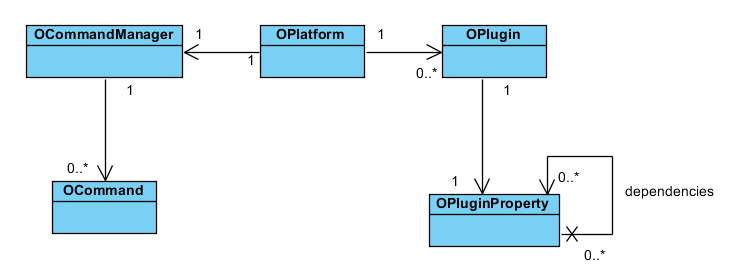
\includegraphics[width=15cm]{figures/class_diagram.png}
\newpage
\section{Installation}

Tout d’abord, dans un terminal, tapez:
\begin{verbatim}
git clone https://github.com/masters-info-nantes/onyx.git
\end{verbatim}

Lorsque tous les fichiers sont téléchargés,vérifiez que le proxy de maven est correct en faisant:
\begin{verbatim}
nano /.m2/settings.xml
\end{verbatim}

Le fichier devrait ressembler à ça:
\begin{verbatim}
<settings>
    <proxies>
        <proxy>
            <id>example-proxy</id>
            <active>true</active>
            <protocol>http</protocol>
            <host>proxy.ensinfo.sciences.univ-nantes.prive</host>
            <port>3128</port>
        </proxy>
    </proxies>
</settings>
\end{verbatim}

Placez-vous dans le dossier où vous avez cloné le projet. 
Tapez la commande:
\begin{verbatim}
mvn clean install
\end{verbatim}

Pour copier tous les plugins dans la plateforme, tapez:
\begin{verbatim}
./mv_jars
\end{verbatim}

Déplacez-vous ensuite dans le dossier onyx-platform:
\begin{verbatim}
cd onyx-platform/
\end{verbatim}

Pour lancer l'execution par défaut, tapez:
\begin{verbatim}
mvn exec:java-X
\end{verbatim}

\newpage
\section{Plugins}

\subsection{Création d'un nouveau plugin}

Un plugin pour être intégré à la plateforme doit, comme vous vous en doutez, implémenter l'interface OPlugin comme ci-dessous:
\subsubsection{myMainClass.java}
\begin{verbatim}
package com.onyx.myPlugin;

import com.onyx.platform.OPlugin;
import com.onyx.platform.OPluginProperty;

public class myMainClass extends OPlugin{

    public myMainClass() {
        //Add some code here
    }

    @Override
    public void onCreate() {
        //Add some code here
    }

    @Override
    public void onStop() {
        //Add some code here
    }

}
\end{verbatim}

Pour que votre plugin soit correctement reconnu par la plateforme, vous devez lui fournir un fichier OManifest sous cette forme:
Attention! Si vous définissez des dépendances pour le plugin, vous devez les inclure dans maven
\subsubsection{OManifest}
\begin{verbatim}
<?xml version="1.0"?>
<manifest>
    <id>com.onyx.myPlugin</id>
    <version>0.1</version>
    <name>myPlugin</name>
    <descriptionplugin for onyx</description>
    <mainClass>com.onyx.myPlugin.myMainClass</mainClass>
    <!--les dépendences ne sont pas obligatoires-->
    <dependencies>
        <dependency>
            <id>com.onyx.core</id>
            <version>${project.version}</version>
        </dependency>
    </dependencies>
</manifest>
\end{verbatim}

Pour ceux qui voudraient se faciliter la vie et utiliser maven pour compiler leurs plugins, voilà un fichier pom.xml basique:
\subsubsection{pom.xml}
\begin{verbatim}
<?xml version="1.0" encoding="UTF-8"?>
<project xmlns="http://maven.apache.org/POM/4.0.0"
         xmlns:xsi="http://www.w3.org/2001/XMLSchema-instance"
         xsi:schemaLocation="http://maven.apache.org/POM/4.0.0 http://maven.apache.org/xsd/maven-4.0.0.xsd">
    <parent>
        <artifactId>onyx</artifactId>
        <groupId>com.onyx</groupId>
        <version>1.0.0-SNAPSHOT</version>
    </parent>
    <modelVersion>4.0.0</modelVersion>

    <artifactId>myPlugin</artifactId>

    <dependencies>
        <dependency>
            <groupId>${project.groupId}</groupId>
            <artifactId>onyx-platform</artifactId>
            <version>${project.version}</version>
            <scope>provided</scope>
        </dependency>
        <dependency>
            <groupId>${project.groupId}</groupId>
            <artifactId>onyx-core</artifactId>
            <version>${project.version}</version>
            <scope>provided</scope>
        </dependency>
    </dependencies>
</project>
\end{verbatim}

\subsection{Déclaration d'une commande}

Chaque plugin peut apporter son lot de commandes avec lui, pour les définir, il suffit d'ajouter le code suivant dans le manifest:

\begin{verbatim}
<manifest>
    ...
    <command>
        <name>My Command</name>
        <id>mycommand</id>
        <usage>this command do some stuff</usage>
        <commandClass>com.onyx.myplugin.command.mycommand</commandClass>
    </command>
</manifest>
\end{verbatim}

\subsection{Déclaration d'un nouveau type de service}
Tout comme les commandes, chaque plugin peut apporter son lot de services avec lui, pour les définir, il suffit d'ajouter le code suivant dans le manifest:
\begin{verbatim}
<manifest>
    ...
    <services>
        <service>com.onyx.core.OAppProperty</service>
    </services>
</manifest>
\end{verbatim}

et la classe service devra contenir certaines annotations pour être interprété

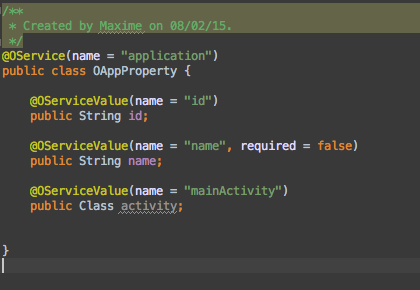
\includegraphics[width=10cm]{figures/newServiceType.png}

\subsection{Déclaration d'un service}

Chaque plugin peut apporter son lot de service avec lui, l'ajout d'une commande est en réalité l'ajout d'un service, son serviceType est quand à lui le seul présent de base dans la platforme. Ainsi le serviceType application est présent dans le core. Pour les définir, il suffit d'ajouter la description de la classe serviceType au manifest, voici un exemple pour le serviceType créé au dessus : 

\begin{verbatim}
<manifest>
    ...
    <application>
        <id>mycommand</id>
        <mainActivity>com.onyx.myplugin.mainActivity</mainActivity>
    </command>
</manifest>
\end{verbatim}
